\section{Introduction}
In recent years, the speed of processors has not increased and the industry has moved towards parallel systems. The only way to increase calculation power is by adding more cores, but this creates higher demand for power and produces more heat. Another way is to take a closer look how our software works. This is exactly the point where we need performance measurement. Without having a clue where the bottleneck is, one does not know how to improve speed. \cite{Jarp2010}

For Linux, performance can be measured with the perf \cite{kernel.org2011} system. It consists of some functionality inside the kernel and a userspace tool called perf. The tool is used to start the measurement in the kernel as also storing and displaying the data. This report will give a detailed description how the data file can be read and the information processed.

\subsection{Performance counters}
Performance counters are often realized as hardware counters. This has the advantages that it has a low overhead and also low perturbation since it does not use registers or the ALU. It is also widespread among different CPUs where it is often called a PMU (Performance Measurement Unit). The PMU can be programmed / configured by the user to count different kind of events. Examples for such events include executed cycles, branch misses and cache misses \cite{Azimi2009}. The basic structure of perf is shown on figure~\ref{fig:perfOverview}.

\begin{figure}[b]
  \center
  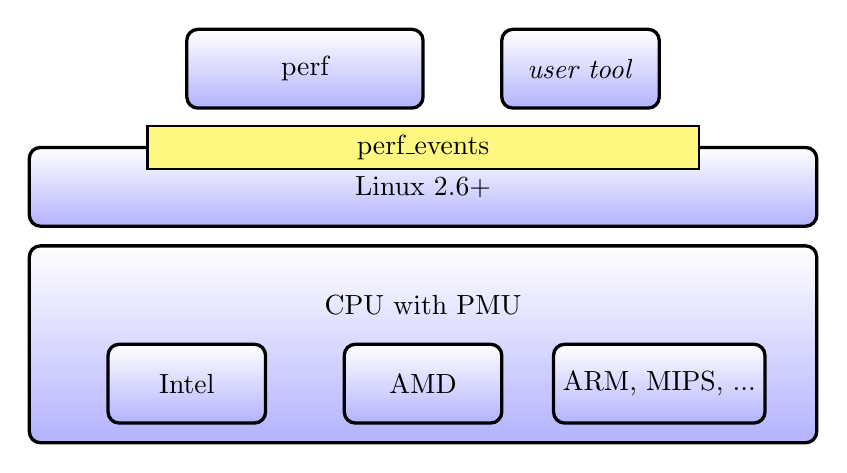
\begin{tikzpicture}[scale=1,transform shape]
\tikzstyle{size}=[minimum width=2 cm, minimum height=1 cm,anchor=center]

\tikzstyle{module}=[size,rectangle,rounded corners,draw=black, top color=white, bottom color=blue!30,very thick, text centered]
\tikzstyle{interface}=[rectangle,draw=black, fill=yellow!50,thick, text centered]
\tikzstyle{label}=[size,rectangle,text centered]

\node [module,minimum width=10 cm,minimum height=2.5 cm] at (0,0.5) (cpu)  {};
\node [label] at (0,1) (cpuLabel) {CPU with PMU};
\node [module] at (-3,0) (intel)  {Intel};
\node [module] at (0,0) (amd) {AMD};
\node [module] at (3,0) (arm) {ARM, MIPS, ... };

\node [module,minimum width=10 cm,minimum height=1 cm] at (0,2.5) (linux)  {Linux 2.6+};
\node [interface,minimum width=7 cm] at (0,3) (perf)  {perf\_events};

\node [module,minimum width=3 cm] at (-1.5,4) (perf)  {perf};

\node [module] at (2,4) (user)  {\textit{user tool}};
\end{tikzpicture}

  \caption[Overview of perf]{Overview of perf. It is based on the Linux kernel interface perf\_events. The Linux kernel needs a CPU with an PMU to measure the hardware. It is also possible to write another performance measurement tool on top of the kernel interface.\label{fig:perfOverview}}
\end{figure}

More information can be found on the level of the hardware \cite{Weaver2011}, focusing on the Linux implementation \cite{Eranian2010}, for an overview of perf \cite{Melo2010} and a workshop which provide an deeper understanding of the PMU \cite{Nowak2011}.

%\todo{rewrite/include} When the event counter overflows, the Instruction Pointer is stored. The matching of the period value to the Instruction Pointer leads therefore not to an exact result. But with a lot of samples the statistically error should decrease.

\subsection{About this document}
The information in this document was gathered with Linux version 2.6.39.3 (9.7.2011, git commit 75f7f9542a718896e1fbe0b5b6e8644c8710d16e). There is no guarantee that the information is valid for different versions.

Different text styles are used to emphasis some content in the document, namely \code{code snippets}, \console{console commands} and \file{files}.

The following terms are used in the described meaning:
\newcommand{\descr}[2]{\item[#1] #2}
\begin{description}
  \descr{event}{a signal produced by the measurement unit, e.g. instruction counter}
  \descr{sample}{an measured occurrence of an event}
  \descr{record}{an entry in the data file, e.g. information about samples or meta information}
\end{description}
